\documentclass[12pt,table,a4paper]{report}

\usepackage{lmodern}
\usepackage[utf8]{inputenc}
\usepackage[T1]{fontenc}
\usepackage{fancyhdr}
\usepackage[french]{babel}
\usepackage[none]{hyphenat}
\usepackage{listings}
\usepackage[nottoc]{tocbibind}
\usepackage{todonotes}
\usepackage{amssymb}
\usepackage[bottom]{footmisc}
\usepackage{graphicx}
\usepackage{wrapfig}
\usepackage{lscape}
\usepackage{rotating}
\usepackage{epstopdf}

\title{TFE: Plateforme de ticketing}
\author{Emmanuel CAPELLE}
\date{}

\DeclareUnicodeCharacter{00A0}{ }
\pagestyle{fancy}
\lhead{}
\renewcommand{\rmdefault}{phv}
\renewcommand{\sfdefault}{phv}
\renewcommand{\headrulewidth}{0.4pt}
\renewcommand{\footrulewidth}{0.4pt}
\setlength{\parindent}{0em}
\setlength{\parskip}{0.5em}
\setcounter{secnumdepth}{3}
% \setcounter{tocdepth}{4}

\begin{document}

\tableofcontents

\newpage

\chapter{Introduction}

\section{État de la question}
Le sujet que je vais aborder dans ce travail de TFE sera la “Conception d’une plateforme de gestion de services d’assistance”.

Il existe sur le web plusieurs solutions, appelées “systèmes de ticketing”, qui répondent à la demande de logiciel de gestion de services d’assistance.

Lors de mon stage en entreprise, j’ai eu pour tâche de développer une application web permettant de gérer en ligne des tickets concernant des appartements habités par les utilisateurs de cette plateforme.

Il existe d’autres exemple de plateformes déjà existantes, tel que "Mantis Bug Tracker"\footnote{https://www.mantisbt.org/}, qui se focalise quant à elle sur l’assistance au développement d’applications informatique.

J’ai abordé ce sujet de TFE avec plusieurs problêmes en tête:
\begin{enumerate}
\item{La vitesse d’exécution du framework utilisé lors de mon stage\footnote{YII: http://www.yiiframework.com/} s’avérait être très lent, malgré l’utilisation rigoureuse des best-practices préconisés par les créateurs dudit framework.}
\item{La flexibilité de ces différentes plateformes reste assez limitée, j’aimerais créer une plateforme extensible dans une certaine mesure, pouvant se "métamorphoser" en une plateforme adaptée aux besoins de ses utilisateurs, via une interface administrateur.}
\item{J’aimerais ajouter une capacité d’ubiquité à ma plateforme en lui ajoutant une application Android permettant de créer et/ou gérer des tickets, peu importe la localisation de ses utilisateurs.}
\end{enumerate}


\section{Délimitation du projet}
Mon projet est constitué de deux parties: d'une part l'application web qui servira d'interface principale à ses utilisateurs, leur permettra de gérer leur compte utilisateur et les paramètres associés à celui-ci ainsi que la création de tickets directement sur le site.

L'accent sera mis sur la communication entre les différents protagonistes pour la résolution de problèmes des utilisateurs de la plateforme. Les différents protagonistes sont les utilisateurs, les gestionnaires de tickets, et les entreprises susceptibles de pouvoir résoudre le problème lié au ticket.

D'autre part, une application android a été créée en tant que support pour l'application web principale. Sa valeur ajoutée est qu'elle permet aux utilisateurs de créer un ticket où qu'ils soient, sans devoir avoir accès à un ordinateur.

\section{Public cible de l'application}
Le public cible de mon projet serait par exemple une entreprise gérant une certaine quantité de bâtiments, dont les habitants seraient les utilisateurs de la plateforme de ticketing. Il serait alors possible de mettre en place une relation utilisateur-gestionnaire et utilisateur-entreprise bien plus facilement.

De plus, il existe différents bénéfices pour les différentes protagonistes à utiliser ma plateforme:

\begin{itemize}
\item{Pour l'utilisateur, le temps de recherche d'une entreprise de confiance serait réduit: les gestionnaires maintiennent à jour une base de données interne à la plateforme, reprenant tous les entreprises partenaires et/ou de confiance. L'utilisateur pourra aussi communiquer facilement avec son gestionnaire de ticket ET l'entreprise en charge de régler le problème lié au ticket.

L'utilisateur peut aussi utiliser la plateforme depuis son smartphone Android, particulièrement utile si un PC n'est pas disponible.}
\item{Pour les gestionnaires, centralisation des tickets de leurs utilisateurs, avec fonction de recherche rapide d'un ticket en particulier. Outils de gestion simple d'utilisation. Communication améliorée via la plateforme de ticketing.}

\item{Pour les entreprises, le fait d'être répertoriée en tant qu'entreprise de confiance sur la plateforme de ticketing pourrait apporter de nouveaux clients à cette entreprise. Possibilité pour l'entreprise de créer un compte sur la plateforme afin de mieux communiquer avec les différents utilisateurs dont elle aurait la responsabilité de résoudre le problème.}
\end{itemize}

\section{Définition de quelques concepts}
\textbf{Service d'assistance}: service offert par l'entreprise propriétaire de la plateforme pour mettre en relation utilisateurs de ladite plateforme et entreprises étant susceptible de résoudre le problème rencontré par l'utilisateur.

\textbf{Ticket}: Un ticket est une demande d'assistance émise par l'utilisateur de la plateforme. Celui-ci est ensuite pris en charge par un gestionnaire de ticket, qui servira d'intermédiaire entre l'utilisateur et une ou plusieurs entreprises.

\textbf{Administrateur}: Dans le cas de cette application, l'administrateur est la/les personnes en charge du backend de l'application. (Base de données, code, ...)

\textbf{Gestionnaire de tickets}: La ou les personne(s) chargée(s) de donner suite aux demandes d'assistance (tickets) émises par les utilisateurs sur la plateforme.

\textbf{Utilisateur}: Est un utilisateur «lambda» de la plateforme, n'ayant aucune permission spéciale dans le système.

\textbf{Django}: Le framework utilisé pour construire la nouvelle plateforme de ticketing.


\chapter{Approche théorique et technique}
\section{Outils et méthodes utilisés}
Environnements de travail:

Développement du site web: IDE PyCharm – community edition de JetBrains\footnote{https://www.jetbrains.com/pycharm/}

Développement de l'app Android: Android studio de JetBrains\footnote{http://developer.android.com/tools/studio/index.html}

Maquettes du site et de l'application Android: Draw.io de JGraph LTD\footnote{https://www.draw.io/}

Diagrammes UML, de séquence, ... : Visual paradigm - community edition de l'entreprise du même nom\footnote{http://www.visual-paradigm.com/}

Écriture de ce rapport: LaTeX\footnote{http://www.latex-project.org/}

\section{Langage de programmation utilisé: Python}
Créé en 1990 par Guido van Rossum, Python est un langage de programmation de haut niveau à typage dynamique, orienté objet et est un langage interprété.

Ce langage à l'avantage d'être portable, et peut fonctionner sur quasiment toutes les systèmes d'exploitation disponibles sur le marché. Si j'ai envie de porter mon application de ticketing sur linux, il est tout à fait possible de le faire, et ce assez facilement.

Python est aussi un langage qui a pris beaucoup de maturité, ce qui a pour avantage d'avoir une assez grande communauté, et par conséquent un choix de librairies assez conséquent.

Simple et direct, Python est particulièrement bien adapté au dévelopement rapide d'applications (RAD).

Il est possible aussi d'interfacer python avec d'autres langages comme C++, java, c\#, etc... Son utilisation est alors plus orientée vers le scripting de comportements.

\begin{center}
Pourquoi ai-je choisi Python? 
\end{center}

Je connais bien Python en tant que langage de programmation. Je l'utilise souvent pour créer des scripts de tout type. C'est un langage très flexible et adaptable à de nombreuses situations.

C'est pourquoi j'ai voulu approfondir ma connaissance de ce langage en lui découvrant une nouvelle facette: La programmation web.

\section{Le framework utilisé: Django}
Django est un framework orienté web créé en 2003 et disponible en version release en juillet 2005. \footnote{Source: http://en.wikipedia.org/wiki/Django\_web\_framework \label{DjangoWikipediaArticle}}.

Ce framework permet le développement non seulement rapide, mais aussi encourageant la modularisation et la réutilisation de modules déjà développés par la communauté. Django intègre les modules de la communauté les plus avancés en termes de fonctionnalités et de performances.

Le framework inclus aussi un outils d'administration flexible et entièrement configurable, je l'ai d'ailleurs personnalisé au niveau de ses fonctionnalités et utilisé dans mon projet.

Voici certains sites web bien connus utilisant Django comme framework de base: Pinterest, Instagram, Mozilla, The Washington Times, Disqus, le Public Broadcasting Service et Bitbucket. \footref{DjangoWikipediaArticle}

\subsection{Pourquoi Django?}

Dans le domaine des frameworks web pour développement rapide de sites web, Django a beaucoup de concurrence (CodeIgniter, Laravel, Yii, ruby on rails, ASP.NET,... Pour ne citer que quelques uns des frameworks les plus connus dans le milieu).

Dans un contexte de popularité du framework par rapport à ses concurrents, Django se place dans le haut du classement (Au moment de l'écriture de ce rapport).\footnote{http://hotframeworks.com/\#top-frameworks}

Il existe de nombreuses offres d'emploi requérant la connaissance de Django, certes, pas autant que d'autres frameworks tel que ASP.NET, mais Django se place de manière très respectable sur le marché du travail.

Finalement, j'ai choisi Django car j'ai voulu apprendre une nouvelle manière de développer une application web, autre que le couramment utilisé PHP et sa pléthore de frameworks disponibles.

\subsection{Fonctionnement de Django}
\subsubsection{Déploiement rapide d'application}
Le déploiement d'une application Django requiert deux choses:

\begin{itemize}
	\item{Une distribution python correctement installée, et préférablement dans sa version 3.x vu les performances améliorées de cette nouvelle version.}
	\item{Les dépendances de librairies python, facilement installées grâce à l'outil PIP qui installe Django et ses dépendances en une seule commande console.}
\end{itemize}

Après avoir installé Python, la librairie Django et ses dépendances, il ne reste qu'à soit cloner un projet Django depuis votre hébergeur git, mercurial ou autre, soit créer un nouveau projet Django.

Django utilise son propre serveur web, pas besoin d'apache pour livrer les pages web aux utilisateurs de la plateforme. Le framework utilise par défaut une base de données SQLite, mais il est facile d'interchanger d'architecture de base de données via le fichier de configuration "settings.py". Il faudra alors obtenir les pilotes adéquats pour pouvoir utiliser le système de base de données sélectionné.

\subsubsection{Architecture web découplée}
Django à comme spécificité d'être très modulable, en effet, il est très facile avec ce framework de pouvoir ajouter un nouveau module à la volée, et ce avec un minimum de configuration.

La seule exigence du framework est que l'application web doit posséder un module de base standardisé et présent d'office lors de la création de l'application web via l'interface en ligne de commande d'administration de Django.

Ce système, très efficace, permet le développement de "plugins"\footnote{Plugin: Extension d'une application principale pour en étendre les fonctionnalités.} et une utilisation rapide de ceux-ci dans des applications existantes.

Par exemple, il est possible qu'une entreprise ai créé son propre système de login sécurisé et réutilisable, il lui est donc très facile d'intégrer ce module dans un projet déjà existant, permettant ainsi de développer plus rapidement de nouveaux modules.

Finalement, la communauté présente autour de Django étant assez grande, il est plus ou moins facile de trouver un module correspondant aux attentes du développeur de la plateforme.

\subsubsection{Architecture MTV}
Les développeurs de Django appellent l'architecture utilisée par Django "`architecture MTV"', pour "Model-Template-View", qui selon leur dires \footnote{https://docs.djangoproject.com/en/1.8/faq/general/ : "`Django appears to be a MVC framework, but you call the Controller the 'view', and the View the 'template'. How come you don’t use the standard names?"'}, diffère par le fait que la vue "décrit quelles données l'on voit, et non pas comment celles-ci sont visibles".

La vue est, somme toute, un fonction appelant un template. La vue passe alors des données au template, qui lui se chargera de les représenter "graphiquement" à l'écran pour l'utilisateur final.

Personnellement, je n'ai pas trouvé cette architecture différente de celle utilisée par MVC, il existe juste cette subtilité décrite ci-dessus, qui ne change au final pas grand chose dans le workflow de développement du site web.

Cette architecture sépare l'application en trois grandes parties, le modèle qui s'occupe de la partie applicative logique, ainsi que des interactions entre la base de données et l'application.

La vue quant à elle sert à définir l'interface homme-machine de l'application, qui permettra à ses utilisateurs de consulter et d'interagir avec les données de l'application.

Pour terminer, le contrôlleur, qui s'occupe de la gestion et de la validation des interactions faites par les utilisateurs via les vues de la plateforme.

Il est à noter que Django utilise une nomenclature propre pour désigner les différentes parties du modèle MVC: Le modèle s'appelle toujours modèle, par contre la vue s'appelera "template", et le contrôleur s'appellera "views", pour cause, le fichier s'occupant de la partie contrôlleur de l'application s'appelle... "views.py". C'est d'ailleurs ce que j'ai trouvé déroutant lorsque j'ai découvert le framework.

\subsubsection{Les modèles}
Les modèles en Django sont tous contenus dans un fichier appelé "models.py". Ce fichier existe dans chacuns des modules existant dans l'application Django.

Les modèles sont représentés par une classe. Ces classes sont consituées de champs (primary key, foreign key, champs normaux,...), mais aussi de méthodes définissant le comportement du modèle, et qui seront appelées par les contrôleurs afin de pouvoir travailler, modifier ou supprimer ces objets.

La création d'objets se fait dans le contrôleur. (voir section sur les contrôleurs, plus bas)

Chacune des classes modèle dérive d'une classe "`Model"' parente, contenant tous les comportements de base d'un modèle. Par exemple: sauvegarde de l'objet dans la DB (via l'ORM), suppression d'un objet, entre autres.

Tous ces comportements sont bien entendu redéfinissables afin de se comporter de la manière la plus adaptée aux besoins du développeur, et donc ultimement aux besoins des utilisateurs.

Il est par exemple possible de redéfinir la méthode "`delete()"' dans le but de passer un champ "`visible"' à faux, au lieu de supprimer la donnée de la base de données. Cette technique est appelée "`soft delete"', et je l'utilise dans mon application.

Cette méthode de découpe des modèles en classes python permet aussi une certaine facilité dans l'écriture de bateries de tests, j'y reviendrai un peu plus tard dans la section consacrée aux tests.

\subsubsection{Les vues}
Tout d'abord, il faut noter une particularité de Django, qui est dûe à son architecture MTV\footnote{Voir chapitre sur l'architecture MTV}: La classe appelée "views.py" est en fait le contrôleur faisant l'interface entre les modèles de l'application, et les templates qui sont, eux, la représentation finale d'une page web. \footnote{Voir chapitre sur les templates}

Il y a deux façons d'aborder la création de vues avec Django:

\begin{itemize}
	\item{Vues fonctionnelles: la vue est alors créée sous la forme d'une fonction, retournant une URL pointant vers un template à faire apparaître à l'écran.}
	\item{Classes vue: La vue est une classe dérivant de la classe parente "TemplateView", la vue devient alors un objet python à part entière, et son comportement peut-être modifié via la redéfinition des méthodes de la classe parente.}
\end{itemize}

Étant donné que les vues dites "fonctionnelles" sont plutôt adaptées aux petits sites web, j'ai choisi d'utiliser exclusivement les classes de vue. En effet, elles donnent accès à l'avantage certain de la flexibilité possible uniquement avec l'orienté objet.

\subsubsection{Comment ces vues fonctionnent-elles?}

Chaque classe de vue est couplée à un template. La différence entre la vue et le template est que la vue se charge de communiquer les données entre le ou les modèle(s) et le template. La fonction de la classe de vue est finalement celle d'un contrôleur normal dans une architecture MVC.

Pour que les utilisateurs puissent atteindre les différentes vues qui composent la plateforme, il est nécéssaire de les lier à une URL unique, c'est alors que le "routeur", aussi appelé "URL dispatcher".

Il existe dans le module racine un routeur de base contenant les instructions de routage de base. L'URL passe d'abord par ce premier routeur qui s'occupe, lui, d'importer la partie de site web requise par l'URL.

Voici le routeur "racine" utilisé par mon application web:
\begin{figure}
	\centering
		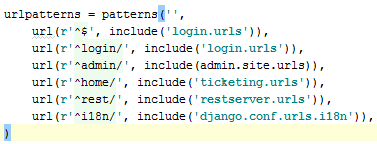
\includegraphics[width=0.8\textwidth,natwidth=377,natheight=144]{images/ticket-routeur-racine.png}
	\caption{Exemple de routeur racine}
	\label{fig:ticket-routeur-racine}
\end{figure}

Les autres modules contiennent aussi un routeur, secondaire celui-ci, qui se charge de déterminer le endpoint\footnote{Endpoint: Destination finale à atteindre \label{endpointFootnote}} à atteindre.

Voici à quoi ressemble un routeur secondaire:
\begin{figure}
	\centering
		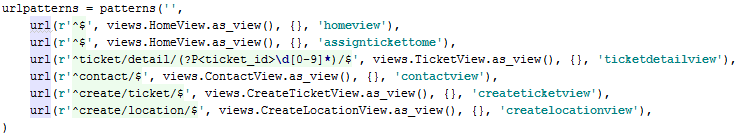
\includegraphics[width=0.8\textwidth,natwidth=737,natheight=136]{images/ticket-routeur-secondaire.png}
	\caption{Exemple de routeur secondaire}
	\label{fig:ticket-routeur-secondaire}
\end{figure}

Une fois cet endpoint\footref{endpointFootnote} déterminé, la vue passe par la méthode d'appel adéquate (GET ou POST) définie dans le header \footnote{Header: en-tête contenue dans toutes les requêtes HTTP.} de la requête.

Les méthodes GET et/ou POST sont surchargées afin de définir le comportement du contrôleur, c'est à cet endroit que se trouve la logique de redirection de l'application. Les méthodes GET et POST doivent obligatoirement retourner un template afin que Django puisse interpréter ce template en page HTML. J'expliquerai ces templates en détail dans la section suivante.

\subsubsection{Les templates}
Un template est un fichier, la plupart du temps au format html, définissant la représentation d'une page web. Un module Django peut contenir un ou plusieurs templates, que le contrôleur de ce module utilisera en fonction des requêtes qui lui sont passées.

Les templates en Django ont la particularité d'être semi-dynamiques, et ce grâce à l'utilisation de variables et de "template tags".

Les variables sont passées par le contrôleur au template via ce que Django appelle les "extras", et sont utilisable dans le template comme une variable python normale. Il est possible d'effectuer des opérations sur ces variables (appel de fonction liée à cette variable) directement dans le template.

La définition d'un "template tag" est quant à elle plus large: Le tag demande au système de template d'effectuer des opérations, prédéfinies dans ce système, tel qu'une condition "IF", une boucle "WHILE", et bien d'autres. Il est aussi possible de définir ses propres "template tags" utilisables dans tous les templates du module Django.

Les templates peuvent être réutilisés via un système d'héritage similaire à l'orienté objet: Un template de base est composé de "blocks", ceux-ci peuvent s'apparenter aux méthodes en orienté objet. Ce template est ensuite étendu par un template enfant qui redéfinira le visuel de ces blocks. Il existe aussi un template tag "block.super" qui appelle la définition du block du parent, ce qui ressemble encore une fois au système d'héritage de l'OO.

Évidemment, ce système n'est pas vraiment de l'orienté objet, vu qu'un template n'est qu'une définition de représentation graphique en HTML de ce que l'utilisateur final verra dans son navigateur.

\missingfigure{Exemple de variable de template et de template tag (screenshot)}

\subsection{L'ORM de Django}
\todo{TODO: L'ORM de Django}
Après avoir écrit les classes modèles, il faut traduire lesdites classes en tables et champs dans la/les base(s) de données utilisée(s) par l'application.

\subsection{SQLite versus MySQL}
SQLite est un type de base de données léger, stocké dans un fichier ".db", ce qui rend cette base de données portable: Un simple copier-coller la relocalise. C'est une très bonne base de données pour tester les applications en développement.

Cependant, SQLite ne possède aucun système de gestion des utilisateurs SQL, de fait il n'y a qu'un seul utilisateur, en tout et pour tout, pouvant effectuer des opérations sur la base de données SQLite.

Cela veut donc dire, aucune connection concurrente possible, et donc perte de performances lors de l'accès à la DB, que ce soit en lecture ou en écriture.

Il est donc sage de penser à la migration depuis une base de donnée type SQLite vers une base de données MySQL, celle-ci prenant en charge la concurrence de plusieurs connections simultanées à ses tables.


\chapter{Implémentation des différentes applications}

\section{Solution de gestion des tickets existante}

\subsection{Présentation du système de ticketing}
Cette plateforme de ticketing a été réalisée lors de mon stage en entreprise.

Le client, que je ne peux pas nommer, avait commandé à l'entreprise dans laquelle j'ai effectué mon stage \footnote{Web3Sys: http://web3sys.com/} une plateforme de ticketing afin de pouvoir gérer les problèmes de leurs utilisateurs de façon centralisée.

Est alors née une application web permettant la gestion de ces tickets, mais lors du développement sont survenus plusieurs problèmes que je vais vous exposer dans la section suivante.

\subsection{Critique de la plateforme existante}
Bien que la plateforme correspondait aux attentes du client, je me suis posé la question, pendant et après mon stage, "comment pourrais-je rendre cette plateforme plus performante et plus flexible qu'elle ne l'est actuellement?".

De plus, nous avions relevé plusieurs soucis lors du développement de l'application:

\begin{itemize}
	\item{L'application ne se basait que sur des catégories et sous-catégories d'incidents, et souvent, une entreprise assignée à tel incident se trouvait beaucoup plus loin géographiquement qu'une autre entreprise pouvant résoudre le même type de problème.}

	\item{Un autre problème que j'ai pu relever lors de mon stage était que la communication entre l'utilisateur et le gestionnaire de son ticket était quasiment nulle, il n'existait que la possibilité d'envoyer un mail à l'entreprise ayant développé l'application, c'est-à-dire mon lieu de stage. Aucune communication possible entre l'utilisateur et l'entreprise se chargeant de résoudre le problème non plus.}

	\item{Les performances au niveau de la vitesse d'exécution de la plateforme laissaient à désirer, il fallait souvent attendre plusieurs secondes avant de pouvoir accéder à la page web désirée, et ce malgré le nombre réduit de "tickets-test". Nous nous étions pourtant conformés aux best practices préconisées par les développeurs de YII\footnote{Le framework utilisé lors de mon stage.}.}

	\item{Finalement, l'architecture mise en place côté plateforme web nous a bloqué lorsque le client nous a demandé de développer un webservice, dans le but de créer une application Android travaillant de paire avec le site web, l'idée d'une application Android a alors été abandonnée.}
\end{itemize}

\section{Conception de la nouvelle solution}
C'est avec les différents problèmes énoncés lors de la section précédente en tête que je me suis mis à développer un système de ticketing et son application Android, tout en utilisant une approche différente de celle adoptée lors de mon stage en entreprise.

\subsection{Approche utilisée lors de la conception de ces applications}
\todo{}

\subsection{Règles métier}
\todo{Compléter les règles métier}
Il est nécéssaire dans ce genre d'applications travaillant avec divers acteurs, qui eux-mêmes travaillent en harmonie pour atteindre un objectif commun (la résolution de problèmes de particuliers), de définir des règles métiers qui assureront le bon fonctionnement de l'application.

Voici les principales règles métier mises en place:

\subsubsection{Administration de la plateforme}
\begin{itemize}
	\item{L'administrateur de la plateforme pourra choisir s'il est possible pour les utilisateurs de la plateforme de s'enregistrer manuellement sur ladite plateforme. Objectif: Filtrage d'éventuelles création de compte intempestive.}
	\item{La création d'entreprises est laissée aux administrateurs et aux gestionnaires, afin de ne pas voir apparaître des entreprises factices.}
	\item{La création de catégories d'évènements est aussi laissée aux administrateurs et aux gestionnaires de la plateforme pour assurer la bonne gestion de ces catégories, ainsi que le lien fait entre une catégorie et une ou plusieurs entreprises.}
	\item{Les utilisateurs et les entreprises sont tenus de mettre à jour leurs informations via la plateforme web, afin que la plateforme puisse déterminer plus précisément les entreprises les plus proches.}
	\item{Les fausses adresses sont à éviter, et sont traitées par le système comme nulles par le système de géolocalisation.}
\end{itemize}

\subsubsection{Gestion des tickets}

\begin{figure}
	\centering
		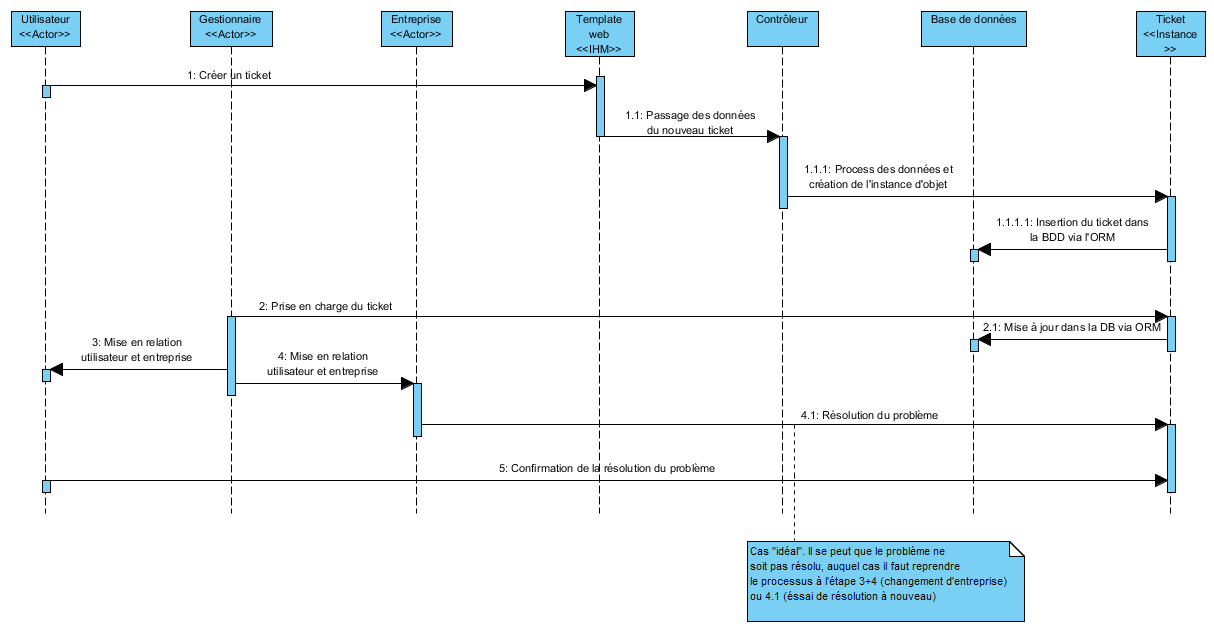
\includegraphics{images/schemas/processus_gestion_ticket.PNG}
	\caption{Processus de gestion d'un ticket}
	\label{fig:processus_gestion_ticket}
\end{figure}


\begin{enumerate}
	\item{Création du ticket par un utilisateur}
	\item{Prise en charge de la gestion du ticket par un gestionnaire de le plateforme}
	\item{Mise en relation entre l'utilisateur et le gestionnaire}
	\item{Passage du ticket au statut "en cours"}
	\item{Assignation d'une entreprise à la résolution du problème lié au ticket, et mise en relation de l'utilisateur, du gestionnaire avec l'entreprise sélectionnée}
	\item{Le problème est-il résolu?
	
	- Oui: poursuivre à l'étape suivante
	
	- Non: revenir à l'étape 4 (changement d'entreprise) ou 6 (nouvelle tentative de résolution du problème) 
	}
	\item{Clôture du ticket}
	\item{Confirmation de la résolution du problème avec les différents protagonistes
	
	- Résolution confirmée par l'utilisateur: Passage du ticket au statut "confirmé"
	
	- Résolution non confirmée par l'utilisateur: Demande d'ouverture d'un nouveau ticket \footnote{Ce système a été choisi afin de garder une trace du ticket, plutôt que de l'écraser.}
	}
\end{enumerate}


\subsection{Flux d'activité de l'application}
\todo{Flux d'activité site web}
\missingfigure{activité PDV utilisateur}
\missingfigure{activité PDV gestionnaire et entreprise}


\subsection{La base de données utilisée par les applications}

\subsubsection{Dictionnaire de données}
Cette partie va vous présenter les différentes données utilisées dans la base de données unique de l'application.
\todo{dictionnaire de données}

\subsubsection{Schéma de la base de données}
Vous trouverez le schéma représentant la base de données dans les annexes, celle-ci étant beaucoup trop volumineuse.

\section{Analyse de l'application Web}
\todo{Sous-sections analyse application web}

\subsection{Librairies utilisées lors du développement de l'application web}
Étant donné la relativement courte durée de développement pour les deux applications, j'ai décidé de m'aider de librairies externes pour différentes tâches qu'il m'aurait été difficile d'implémenter, par rapport au manque de temps, soit au manque de connaissances sur le sujet.

\subsubsection{Design de base avec bootstrap}
N'étant pas un pro du design web, j'ai utilisé "bootstrap" \footnote{Bootstrap: http://getbootstrap.com/} pour donner à mon application web un design assez léger, tout en étant fonctionnel et facile à implémenter, et ce même sur une application déjà operationnelle.

\missingfigure{Insérer un aperçu visuel de ce que bootstrap produit (taille réduite)}

\subsubsection{JQuery}
Travaillant main dans la main avec javascript, "JQuery" est une librairie d'extensions en javascript qui permettent d'étendre, ou du moins de simplifier, l'implémentation de comportements en javascript.

La partie commentaire de la vue ticket est un exemple d'utilisation de JQuery: le <div> est rétractable et extensible à souhait, et grâce à JQuery, l'implémentation de ce comportement est très simplifiée (voir figure \ref{fig:jquery-collapse-extend-div}) comparé à une implémentation exclusivement en javascript.

\begin{figure}[htbp]
	\centering
		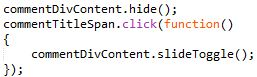
\includegraphics{images/code-snippets/jquery-collapse-extend-div.JPG}
	\caption{Exemple d'accordéon en JQuery}
	\label{fig:jquery-collapse-extend-div}
\end{figure}

\subsubsection{Geolocalisation}
L'un des problèmes rencontrés lors de mon stage était que l'entreprise assignée par un gestionnaire de ticket pouvait très bien se trouver à des centaines de kilomètres de l'endroit désigné par l'utilisateur dans son ticket.

J'ai alors trouvé une solution à ce problème en calculant la distance entre le lieu spécifié dans le ticket et les entreprises contenues dans la base de données de l'application. Si l'entreprise ne possède pas d'adresse, ou possède une adresse invalide, celle-ci aura une valeur de distance très grande, hardcodée à 99999km dans le code.

Si par contre le bâtiment lié au ticket ne possède pas d'adresse, ou possède une adresse invalide, aucune géolocalisation ne sera alors possible, et toutes les entreprises auront la même valeur de distance (toujours 99999km).

Je suis parvenu à un résultat en utilisant l'API Google maps, mais cette API étant limitée en nombre de requêtes journalières, j'ai dû implémenter un premier tri:

\begin{itemize}
	\item {J'ai ajouté aux entreprises des catégories d'incident que celles-ci sont susceptibles de pouvoir gérer.}
	\item {Au lieu de géolocaliser toutes les entreprises de la base de données, j'ai implémenté un filtre ne prenant en compte que les entreprises pouvant résoudre le problème lié au ticket en cours.}
	\item {Finalement, j'ai trouvé une librairie en Python, appelée GeoPy \footnote{GeoPy: https://github.com/geopy/geopy}\footnote{documentation de GeoPy: https://geopy.readthedocs.org/en/1.9.1/} permettant d'utiliser plusieurs services de géolocalisation à la fois, ce qui non seulement relève assez fortemement la limite de requêtes journalières, mais augmente la vitesse de traitement de la géolocalisation.}
\end{itemize}

La géolocalisation a été très facilitée grâce à GeoPy, il ne me restait alors qu'à effectuer une requête par entreprise et à récupérer la liste des entreprises, triée par distance, et à envoyer cette liste au contrôleur.

Sur la vue navigateur, la dropdown list de sélection d'un entreprise pour assignation au ticket sera remplie avec les valeurs reçues du contrôleur. (voir figure \ref{fig:dropdown-selection-entreprise})

\begin{figure}[hb]
	\centering
		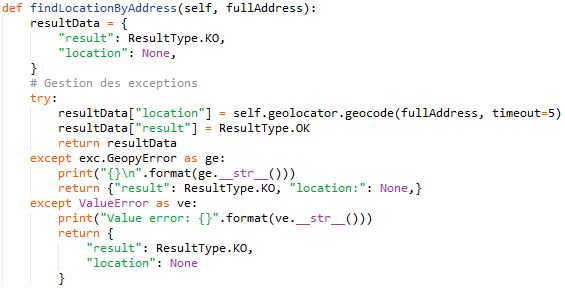
\includegraphics{images/code-snippets/geolocalisation-findlocationbyaddress.JPG}
	\caption{Trouver une localisation par adresse}
	\label{fig:geolocalisation-findlocationbyaddress}
\end{figure}

\begin{figure}[hb]
\centering
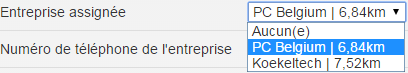
\includegraphics{images/screenshots/web/dropdown-selection-entreprise.png}
\caption{Exemple de sélection d'entreprise}
\label{fig:dropdown-selection-entreprise}
\end{figure}


\subsection{Analyse de l'architecture logicielle}

\subsubsection{Les modèles utilisés par l'application}
\todo{}


\subsection{Le web service avec REST}
Pour permettre la communication avec les différents clients mobiles Android, j'ai décidé d'utiliser l'architecture REST.

\subsubsection{Qu'est-ce que l'architecture REST?}
% http://en.wikipedia.org/wiki/Representational_state_transfer
REST, ou \textit{REpresentational State Transfer}, est une architecture reprenant les best practices en matière de création de web services évolutif.\footnote{http://en.wikipedia.org/wiki/Representational\_state\_transfer}

Cette architecture est composée d'une série de contraintes; j'ai répertorié celles qui m'ont le plus interessé lors du développement de mon web service:

\begin{itemize}
	\item{La contrainte "Client-Server": Le client (l'application Android dans mon cas) et le serveur (le web service développé à côté du site web principal) communiquent entre eux via une interface unique et flexible, présente du côté du web service.
	
	Ce client permet, par exemple, de ne pas se préoccuper du stockage des informations (un ticket, un bâtiment, etc...) en local, mais laisse plutôt le serveur présent en amont du web service du stockage desdites données. De la même manière, le serveur ne s'occupe pas de la présentation (interface utilisateur) de ces données, car c'est l'application cliente qui s'en occupe.
	
	Cette contrainte permet aussi la réutilisation du web service par d'autres clients. J'aurais pû par exemple développer une application visant les téléphones mobiles tournant sous iOS, tout en gardant le code du web service inchangé.}
	\item{La contrainte "Stateless": Cette contrainte signifie que toute requête passant entre le web service et le client reprennent l'intégralité des informations nécéssaires au traitement de cette requête.
	
	Ainsi, le contexte client\footnote{"Le client est-il connecté?", "Quelle est la dernière requête qu'il m'a envoyée?" } n'a pas a être stocké par le web service.
	
	Pour définir quel utilisateur a envoyé la requête au web service, des informations de session sont envoyées à chacune de celle-ci. J'ai personnellement opté pour un système de token, permettant de donner l'autorisation d'effectuer des tâches via le web service que si ce token est existant et valide.}
	\item{La contrainte d'"interface uniforme": qui elle est composée de quatre sous-contraintes, deux d'entre elles ayant été plus importantes lors du développement de mon web service:
			
			1. "Identification des ressources": La ressource à utiliser est identifiée via l'URL précisé dans la requête envoyée par l'utilisateur. En Django, cela fonctionne de la même manière qu'un routeur de vues. (voir figure \ref{fig:exemple-routeur-webservice})
			
			2. "Manipulation des ressources via représentations": Le client a le pouvoir de modifier, créer, supprimer une instance de modèle Django via les données qui lui ont été fournies par le web service, celui-ci faisant office d'intermédiaire entre le client et les modèles Django. Le web service remplace en quelque sortes le contrôleur Django.}
\end{itemize}

\begin{figure}
	\centering
		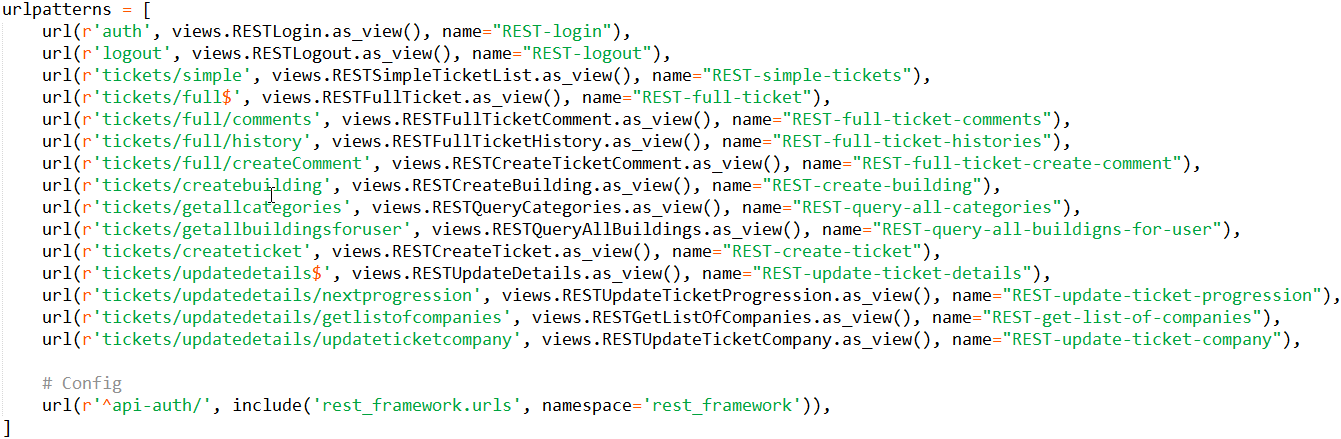
\includegraphics[width=0.90\textwidth]{images/code-snippets/exemple-routeur-webservice.png}
	\caption{Routeur du web service}
	\label{fig:exemple-routeur-webservice}
\end{figure}

\subsubsection{Implémentation du web service aux côtés Django}
J'ai implémenté mon web service à côté de Django. Celui-ci ne fait pas partie intégrante de l'application web, mais communique avec elle via une librairie\footnote{Django Rest Framework: http://www.django-rest-framework.org/} permettant, entre autres, de faire la liaison entre un objet sérialisé par Django Rest Framework et un modèle normal, présent dans l'implémentation du site web en Django.(voir figure \ref{fig:communication-django-webservice-android})

\begin{figure}
\centering
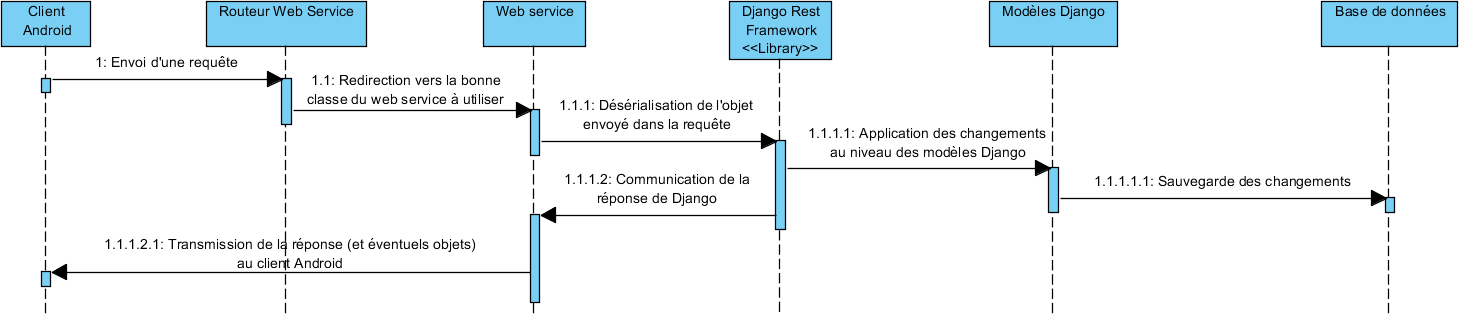
\includegraphics[width=0.9\textwidth]{images/schemas/communication-django-webservice-android.png}
\caption{Schéma de la communication entre le client et Django via web service}
\label{fig:communication-django-webservice-android}
\end{figure}

\subsubsection{Dissection d'une requête REST}
Les requêtes REST utilisées par mes applications sont créées au format HTTP, ces requêtes sont composées de plusieurs parties:

\begin{itemize}
\item L'URI\footnote{\textit{Uniform Resource Identifier}} à atteindre dans le web service, par exemple "127.0.0.1/rest/liste-des-tickets". Cette URI est traduite par le routeur du web service afin d'atteindre la bonne classe
\end{itemize}



\section{Analyse de l'application Android}

\subsection{Pourquoi une application Android?}
\todo{Pourquoi une application android?}
Dans un monde où la population bouge beaucoup, il est important pour une application de pouvoir être disponible n'importe où, et à n'importe quel moment.

Cette application permet aux utilisateurs de la plateforme de pouvoir gérer et être mis à jour de l'avancement de son ou ses ticket(s) en cours.



\subsection{Analyse de l'application conçue}

\subsubsection{Architecture générale}
L'architecture de mon application Android est fortement découplée: J'ai implémenté les différentes activités de manière à ce qu'elles communiquent entre elles via un bus d'évènement, plutôt que de passer des données en paramètre à la création de ces activités.

\missingfigure{schéma montrant l'UML des activités}

\subsubsection{Système de pseudo-cookie pour le login}
Lors du login, l'utilisateur doit entrer ses informations (email et mot de passe) afin de pouvoir accéder aux différents services proposés par l'application Android.

Afin d'éviter que cet utilisateur ne doive entrer ces informations à chaque utilisation de l'application, j'ai mis en place un système de pseudo-cookie.

Sur la vue de l'activité de login se trouve un bouton "remember me". Si celui-ci est coché, l'application écrira les informations de login en clair dans un fichier interne localisé dans le cache de l'application; ce cache se trouve dans la partie "root" de l'OS android, et est donc accessible si l'utilisateur possède un appareil "rooté".

Afin d'assurer une relative sécurité aux informations de login de l'utilisateur, si celui-ci décide de ne pas cocher l'option "remember me", le fichier contenant ces informations sera effacé du cache de l'application, afin d'éviter un éventuel accès à ces données personnelles.

Ce système fonctionne bien, mais n'assure pas une sécurité optimale. Une idée à développer serait, par exemple, le hashage du mot de passe avant son écriture dans le fichier.

\subsubsection{Système de cache en mémoire}
\todo{}
J'ai implémenté dans l'application un système de cache permettant de stocker, entre autres, un ticket complet, une liste de tickets "simplifiés", les informations de l'utilisateur récupérées via le web service, etc...

Le but de ce système de cache est de limiter les transactions entre le client Android et le web service, et ce dans une optique de réduction d'utilisation du réseau\footnote{Voir aussi \ref{sssec:minimisation-utilisation-reseau}}, dans le but:

\begin{itemize}
\item{D'optimiser la vitesse d'exécution des transactions entre le web service et ses clients Android}
\item{De réduire l'utlisation de la bande passante pour les utilisateurs se servant de la 3G/4G comme connection internet}
\end{itemize}

\begin{center}
Fonctionnement du système de cache en mémoire
\end{center}

Prenons le cas des informations de l'utilisateur, comprenant sa primary key dans la base de données, son token d'autentification, son email, son mot de passe, etc... Il est important de connaître ces informations à tout moment dans l'application Android, afin de pouvoir assurer une bonne communication entre l'utilisateur et le web service.

Il est impensable que l'utilisateur doive se reconnecter entre chaque changement d'activité, l'ergonomie de l'application s'en verrait fortement réduite. C'est pour cela qu'une fois l'utilisateur connecté à l'application, celle-ci reçoit du web service les informations complètes de l'utilisateur, et les stocke directement dans son propre cache.

Un autre exemple est le cache contenant les informations d'un ticket complet, en vue de leur utilisation dans une vue détaillée du ticket. Encore une fois, il est important de garder les informations du ticket, car:

\begin{enumerate}
\item{L'application a besoin de ces informations dans plusieurs vues et fragments différents.}
\item{L'utilisateur est susceptible de rester un certain temps sur la vue détaillée d'un ticket, car celui-ci est sensé être préoccupé de l'état d'avancement du ticket qu'il a ouvert.}
\end{enumerate}

Lors d'une requête des détails d'un ticket, l'application va d'abord vérifier si le ticket demandé, identifié via son code ticket unique, n'est pas déjà présent dans le cache. Si ce n'est pas le cas, un requête est effectuée via le client REST, et le résultat de celle-ci sera stocké en cache. Sinon, si le ticket complet est déjà en cache, aucune requête n'est effectuée et les informations seront directement chargées du cache dans la vue détaillée du ticket.

\begin{center}
Problème de ce système de cache
\end{center}

Lors de l'écriture de ce rapport, je me suis posé la question \textit{"Et si un autre utilisateur avait modifié le ticket, et que le cache ne reflétait pas la réalité du ticket?"}.

À cette question, je me suis dit que le ticket ne serait de toute façon pas corrompu si un requête de modification sur celui-ci avait été faite.

Mais il reste le problème que l'utilisateur de l'application Android ne voit pas les informations mises à jour du ticket. À ce problème, j'ai eu l'idée d'implémenter une méthode de hashing, comprenant toutes les informations ticket.

L'idée aurait été de comparer le hash du ticket possédé par le cache du client à celui contenu dans la base de données du site web en Django. Cela aurait permis de comparer de façon quasi\footnote{Attention aux collisions générées par la méthode de hash!} certaine la similitude entre le ticket contenu dans le cache Android et celui contenu dans la base de données Django.

Cependant, par manque de temps, je n'ai pas pu implémenter cette solution dans mon application.

\missingfigure{Code cache}


\subsubsection{Mise en place d'un bus d'évènements}
Tout a commencé lorsque j'ai voulu émettre une requête de login via mon client REST, depuis mon activité "login". L'application envoyait bien une requête vers le web service, mais attendait la réponse qui, bien que quasiment instantanée, bloquait mon application pendant quelques millisecondes.

Je me suis alors rendu compte que j'envoyais mes requêtes REST depuis le thread principal de mon application, ce qui expliquait pourquoi celle-ci se gelait à chaque requête effectuée par celle-ci.

M'est alors venue l'idée d'implémenter un système de requête REST lancées depuis un "worker"\footnote{Un "worker" est un thread à durée de vie très limitée dans le temps, permettant l'exécution d'un tâche en dehors du thread principal, et retournant une réponse à celui-ci.}, mais je me suis rapidement rendu compte que cette tâche était loin d'être triviale et que je n'aurais probablement pas assez de temps pour terminer l'implémentation de ce système à temps.

C'est alors que j'ai trouvé la librairie "Otto"\footnote{http://square.github.io/otto/}, permettant la communication asynchrone entre différentes parties de l'application Android, ainsi qu'une communication avec la librairie "Retrofit" permettant d'émettre des requêtes REST vers le web service.

\begin{center}
Comment fonctionne Otto?
\end{center}

\todo{}
% http://vinsol.com/blog/2014/11/04/communication-patterns-for-application-components/


\subsection{Flux d'information entre le webservice et l'application Android}
\todo{Flux d'information android}


\subsubsection{Minimisation de l'utilisation réseau des requêtes REST} \label{sssec:minimisation-utilisation-reseau}
Lors du développement de mon application Android, je me suis posé la question du problème de la taille des requêtes REST, et de son impact sur les performances globales de l'application android et du web service.

J'ai trouvé deux solutions à ce problème:


\subsubsection{Compression de requête REST}
Avant l'envoi d'une requête REST, il faut compresser le corps de celle-ci via la méthode GZIP, et ainsi en réduire la taille. Il existe cependant un problème, car Django et plusieurs autres web services ne savent pas gérer les requêtes REST compressées avec la méthode GZIP.


\subsubsection{Utilisation de "modèles réduits"}
Au lieu d'échanger des instances entières d'objets et leurs sous-objets\footnote{Un modèle ayant une foreign key vers un autre modèle génère un "sous-objet", lié par composition à l'objet principal.} entre le web service et l'application Android, ceux-ci échangeront plutôt des instances "distillées" d'objets, ne reprenant que les informations nécéssaires à la transaction entre le client Android et le web service.

Par exemple, lors de l'affichage de la liste des tickets de l'utilisateur, seuls la primary key, le statut et le code ticket sont passés au client REST Android, ce qui diminue considérablement la taille des requêtes réseau.

Sur la figure \ref{fig:rest-full-ticket}, vous pouvez voir que la requête pèse 17109 bytes (soit \textbf{\textasciitilde17,11kB}) quand le web service retourne une liste de tickets complets. 

Par contre, la même requête (cache du client Android vidé) mais à laquelle le web service répond par une liste de tickets "distillés", ne comprenant que les informations essentielles, ne pèse plus que 6193 bytes (soit \textbf{\textasciitilde6,2 kB}) (voir figure \ref{fig:rest-simple-ticket}), ce qui correspond à une réduction de \textbf{\textasciitilde63,7\%} de la taille de la transaction réseau.

Bien entendu, le nombre de tickets reste assez limité dans mon application, mais imaginez l'impact d'une telle réduction de taille de transaction réseau lors de l'utilisation de cette application par plusieurs dizaines de clients Android concurrents, à savoir qu'une telle plateforme, telle que je l'ai pensée, devrait pouvoir être capable de soutenir plusieurs dizaines de clients simultanés.

Il y a par contre un petit désavantage à cette pratique, c'est la multiplication des classes de modèle du côté Android, ainsi que des sérialiseurs côté web service. Cependant, au vu des résultats, je pense qu'une augmentation de la taille du code vaut vraiment le coup d'être implémentée. 

\begin{figure}[t]
\centering
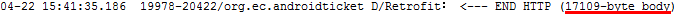
\includegraphics[width=1.0\textwidth]{images/screenshots/proofs/comparaison-rest-full-ticket.png}
\caption{Taille de la requête avec objets complets}
\label{fig:rest-full-ticket}
\end{figure}

\begin{figure}[t]
\centering
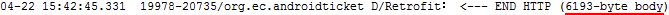
\includegraphics[width=1.0\textwidth]{images/screenshots/proofs/comparaison-rest-simple-ticket.png}
\caption{Taille de la requête avec objets simplifiés}
\label{fig:rest-simple-ticket}
\end{figure}

\subsection{Flow de l'application Android}
\todo{flow de l'application android}
Cette section va parler du flow suivi par un utilisateur et par un gestionnaire lorsqu'il utilise l'application Android.

\missingfigure{Flow app android}


\subsection{Client REST}
Le client REST, implémenté dans l'application Android grâce à la librairie "Retrofit"\footnote{http://square.github.io/retrofit/}, fait office d'interface entre l'application Android et le web service, implémenté dans le cas de ce projet aux côtés de mon site web Django.

L'utilisation principale de ce client REST est l'échange de données entre les deux applications, que ce soit une simple requête de données ou la création d'un nouveau ticket, par exemple.

Je vous invite à lire la sous-section "Qu'est-ce que l'architecture REST?", vous y trouverez une explication du fonctionnement de REST.

\subsubsection{Comment fonctionne la librairie "Retrofit"}
\todo{}

\section{Autocritique de la nouvelle solution mise en place}
\subsection{Résolution des problèmes posés}
\subsubsection{Performances du site web et de l'application Android}
\subsubsection{Flexibilité de l'application}
\subsubsection{Accessibilité à la plateforme}

\chapter{Conclusion}
\todo{conclusion}

\chapter{Annexes}


\section{Schéma de la base de données}
Attention: Ce schéma ne reprend que les tables importantes pour l'application développée. Il existe d'autres tables propres à Django, mais je ne les ai pas incluses car le schéma serait bien trop imposant.

\begin{sidewaysfigure}
\centering
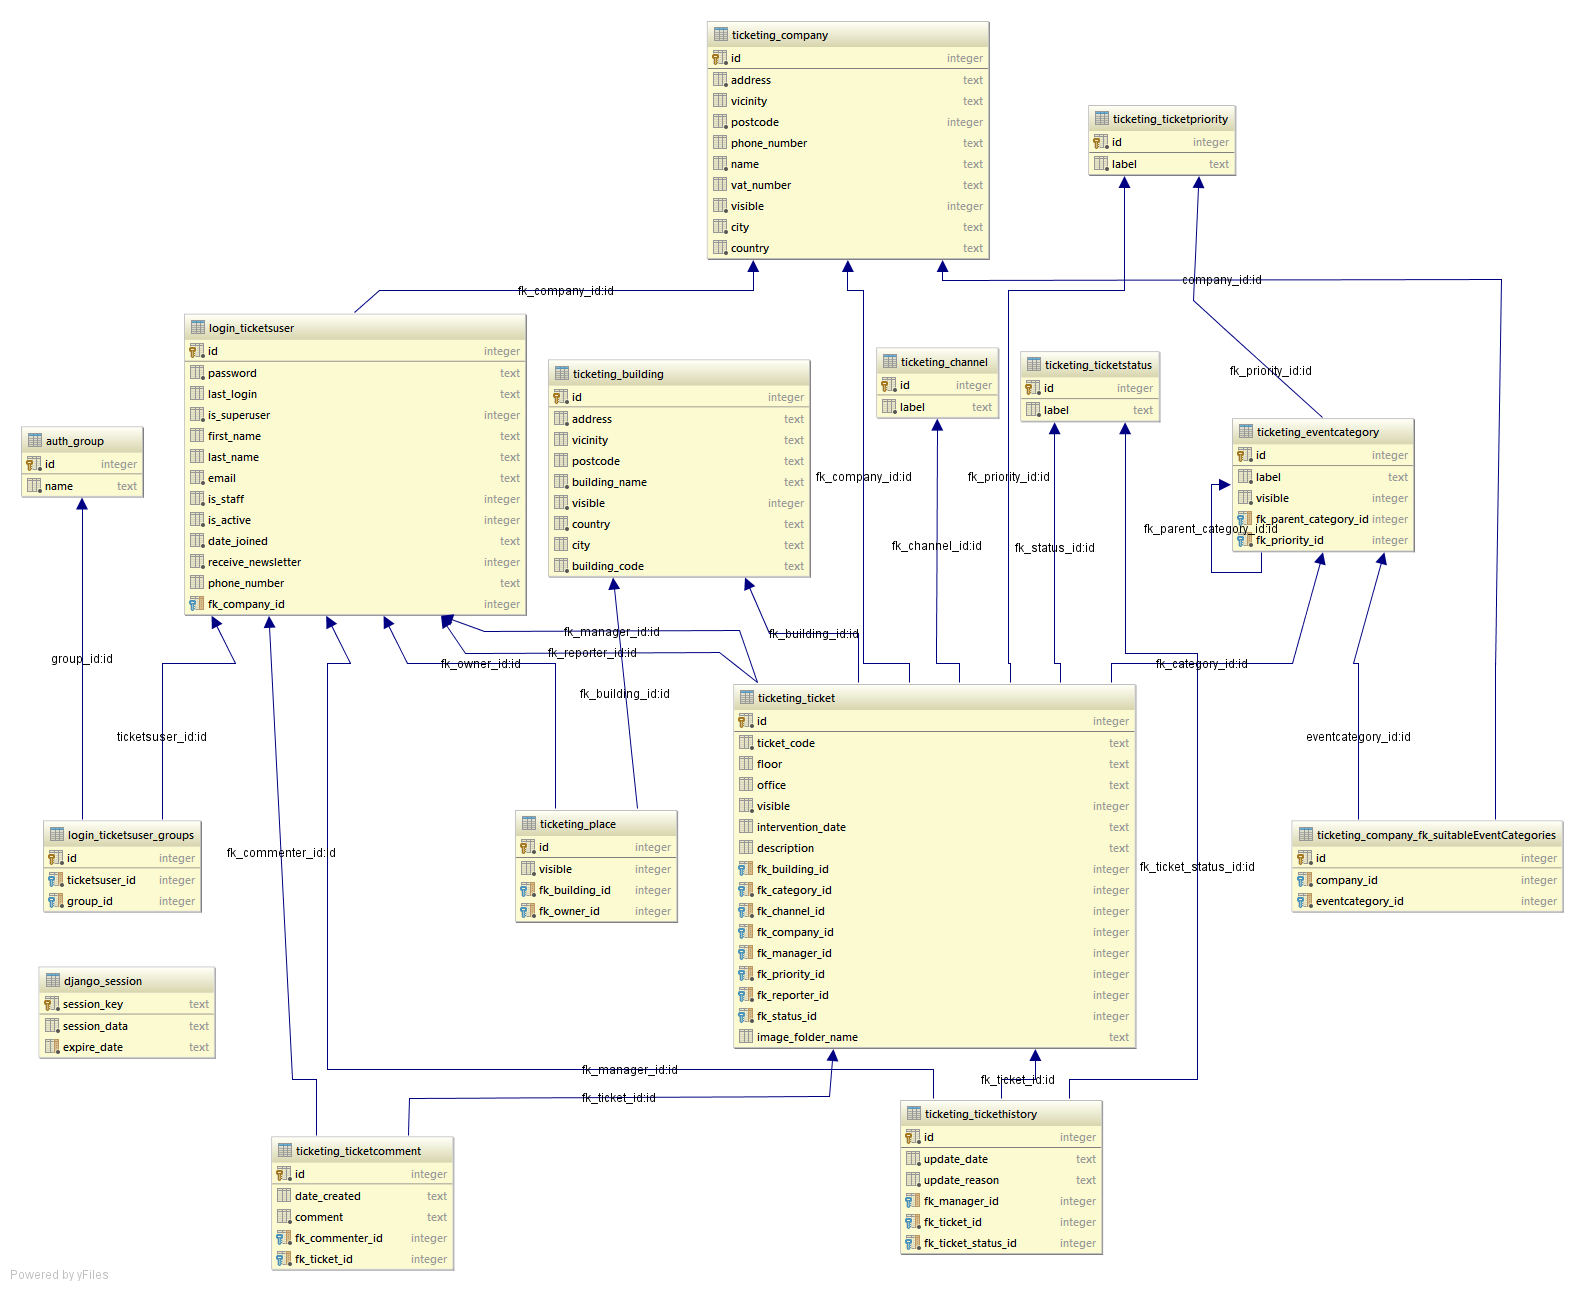
\includegraphics[width=\textwidth]{images/schemas/ticket-database-schema.png}
\caption{Schéma de la base de données de l'application}
\label{fig:schema-database}
\end{sidewaysfigure}



\begin{thebibliography}{breitestes Label}
	\bibitem{How to tango with Django}
	    How to tango with Django
	    
	    http://en.wikibooks.org/wiki/LaTeX/List\_Structures
	
	\bibitem{Documentation Django online}
		Documentation Django online
		
		https://docs.djangoproject.com/en/1.8/
	
	\bibitem{Django Book (online)}
	    Django Book
	    
	    http://www.djangobook.com/en/2.0/
	    
	    Note: En partie obsolète, mais je l'ai utilisé pour apprendre les bases de Django
	    
	\bibitem{How do Django class-based views work?}
			How do Django class-based views work?
			
			http://www.gregaker.net/2012/apr/19/how-do-django-class-based-views-work/
			
	\bibitem{Wikipedia}
			Wikipedia
			
			http://en.wikipedia.org/wiki/Django\_\%28web\_framework\%29
\end{thebibliography}

\end{document}
